% D7065E Final Report — Fire Detection & Autonomous Response
% Based on the course template (final_report_template.tex)

\PassOptionsToPackage{unicode}{hyperref}
\PassOptionsToPackage{hyphens}{url}
\PassOptionsToPackage{dvipsnames,svgnames,x11names}{xcolor}

\documentclass[11pt]{article}
\usepackage{amsmath,amssymb}
\usepackage{lmodern}
\usepackage{iftex}
\ifPDFTeX
  \usepackage[T1]{fontenc}
  \usepackage[utf8]{inputenc}
  \usepackage{textcomp}
\fi
\IfFileExists{microtype.sty}{\usepackage[]{microtype}\UseMicrotypeSet[protrusion]{basicmath}}{}

\makeatletter
\@ifundefined{KOMAClassName}{%
  \IfFileExists{parskip.sty}{\usepackage{parskip}}{%
    \setlength{\parindent}{0pt}\setlength{\parskip}{6pt plus 2pt minus 1pt}}
}{\KOMAoptions{parskip=half}}
\makeatother

\usepackage{xcolor}
\IfFileExists{xurl.sty}{\usepackage{xurl}}{}
\IfFileExists{bookmark.sty}{\usepackage{bookmark}}{\usepackage{hyperref}}
\hypersetup{
  pdftitle={Fire Detection \& Autonomous Response, Architecture Document},
  pdfauthor={Binay Mishra},
  colorlinks=true,
  linkcolor={RoyalBlue},
  filecolor={Maroon},
  citecolor={Blue},
  urlcolor={Blue}}
\urlstyle{same}

\usepackage[a4paper,margin=2.4cm]{geometry}
\usepackage{longtable,booktabs,array}
\usepackage{calc}
\usepackage{graphicx}
\usepackage{float}

\makeatletter
\def\maxwidth{\ifdim\Gin@nat@width>\linewidth\linewidth\else\Gin@nat@width\fi}
\def\maxheight{\ifdim\Gin@nat@height>\textheight\textheight\else\Gin@nat@height\fi}
\makeatother
\setkeys{Gin}{width=\maxwidth,height=\maxheight,keepaspectratio}

\setlength{\emergencystretch}{3em}
\providecommand{\tightlist}{\setlength{\itemsep}{0pt}\setlength{\parskip}{0pt}}
\setcounter{secnumdepth}{-\maxdimen}

\usepackage{newunicodechar}
\usepackage{textcomp}
\usepackage{amssymb}
\newunicodechar{°}{\textdegree}
\newunicodechar{→}{\ensuremath{\rightarrow}}
\newunicodechar{≤}{\ensuremath{\leq}}
\newunicodechar{≥}{\ensuremath{\geq}}
\newunicodechar{≈}{\ensuremath{\approx}}
\newunicodechar{✓}{\ensuremath{\checkmark}}
\newunicodechar{–}{--}
\newunicodechar{—}{---}

\usepackage{etoolbox}
\AtBeginEnvironment{longtable}{\footnotesize}
\AtBeginEnvironment{tabular}{\footnotesize}

\usepackage{fancyhdr}
\pagestyle{fancy}\fancyhf{}
\rhead{\small D7065E\,--\,Architecture Document}
\lhead{\small Fire Detection \& Autonomous Response}
\cfoot{\thepage}
\renewcommand{\headrulewidth}{0.4pt}

\usepackage{titlesec}
\titleformat{\section}{\Large\bfseries}{\thesection}{0.6em}{}
\titleformat{\subsection}{\large\bfseries}{\thesubsection}{0.5em}{}

\usepackage{microtype}
\usepackage{pgfplots}
\pgfplotsset{compat=1.16}
\setlength{\emergencystretch}{2em}

\usepackage{listings}
\lstset{
  basicstyle=\ttfamily\small,
  breaklines=true,
  frame=single,
  backgroundcolor=\color{gray!10},
}

% Placeholder for diagrams
\newcommand{\diagramslot}[1]{\par\begin{center}\fbox{\parbox[c][3cm][c]{0.82\linewidth}{\centering\textit{[Insert: #1]}}}\end{center}\par}

\begin{document}

\begin{center}
{\LARGE Fire Detection \& Autonomous Response\par}
\vspace{0.5em}
{\large D7065E, Architecture Document\par}
\vspace{1em}
{Group 3: Binay Mishra\par}
\end{center}

\vspace{1.2em}

{
\hypersetup{linkcolor=black}
\setcounter{tocdepth}{3}
\tableofcontents
}

\newpage

%% ============================================================================
\section{1. Summary}
%% ============================================================================

This system detects fire events in the A-Building at LTU and responds autonomously: it senses smoke, carbon monoxide, and temperature in every room; an LLM-powered agent decides whether a fire is real, which sprinklers to activate, and which fire doors to unlock; and evacuation routes are computed avoiding affected zones. The building itself, its 950 rooms across three floors, sensors, actuators, and 3D view, is provided by BuildSim, which holds the shared building state; this project provides the physics simulation, the sensor degradation, the intelligence, and the autonomous response around it. The guiding principle is \textbf{detect early, respond building-wide, degrade gracefully}: a fire on any floor triggers a response across all floors, and if the LLM is unavailable, rule-based fallback keeps the building safe.

\begin{longtable}[]{@{}
  >{\raggedright\arraybackslash}p{(\columnwidth - 2\tabcolsep) * \real{0.35}}
  >{\raggedright\arraybackslash}p{(\columnwidth - 2\tabcolsep) * \real{0.65}}@{}}
\toprule
\textbf{Field} & \textbf{Value} \\
\midrule
\endhead
\textbf{Project title} & Fire Detection \& Autonomous Response \\
\textbf{Team members} & Binay Mishra (Group 3, solo) \\
\textbf{Use case} & Autonomous fire detection, response planning, and building-wide evacuation \\
\textbf{Repository} & \url{https://github.com/applied-ai-ltu/d7065e} \\
\textbf{Version / date} & v1.0 / 2026-10-12 \\
\bottomrule
\end{longtable}

\textbf{Changes since the proposal.} Three design changes were made because the evidence demanded it. First, the proposal planned GEPA (Guided Evolutionary Prompt Architecture) for self-improving prompts; on real data it added complexity without measurable benefit over a well-crafted static prompt with verification, so the agent was kept as a two-stage assess-then-verify pipeline and the time was invested in graceful degradation and ClearML-managed retraining instead. Second, the proposal planned Grafana control buttons using the Business Forms plugin; after extensive testing the plugin's state management proved incompatible with simple button use cases, so fire control was moved to a standalone FastAPI API with Swagger UI, and Grafana became monitoring-only. Third, the proposal scoped monitoring to a single room; the architecture naturally scaled to 950 rooms across three floors once the sensor gateway was parameterised by level, so the scope was expanded to demonstrate full-building coverage.


%% ============================================================================
\section{2. Use case and building context}
%% ============================================================================

\textbf{The building.} The system controls the A-Building at LTU, modelled in BuildSim across three floors: level0 (318 rooms, 45 corridors), level1 (351 rooms, 49 corridors), and level2 (287 rooms, 38 corridors), totalling 950 uniquely-named spaces. BuildSim is the shared state of the cyber-physical system: it owns the building model (rooms, levels, equipment), exposes a REST API to register devices and to read and write their state, provides a navigation graph per floor and cross-floor stairwell edges, and streams live state to a 3D web viewer over WebSocket. BuildSim is not modified; it is instrumented. This separation is deliberate---it is exactly the seam between the physical half of a CPS (the building, behind BuildSim's API) and the cyber half (this project's processes), and keeping that seam clean is what would let the same software later drive a real building instead of a simulated one.

\textbf{How the system connects to BuildSim.} Each of the project's processes talks to BuildSim through its REST API, and nothing else touches the building state directly:
\begin{itemize}\tightlist
  \item The \textbf{physical simulator} reads actuator state from BuildSim (GET), advances the room physics (heat, smoke, CO propagation), and writes the resulting sensor values back into BuildSim (PUT /api/sensors/\{id\}/value). This is what closes the feedback loop.
  \item The \textbf{sensor gateway} reads those values from BuildSim, degrades them with noise, lag, drift, and stuck-sensor failures, and publishes to the MQTT broker, so the pipeline and agent can consume them independently.
  \item \textbf{Actuators} are registered in BuildSim. The agent commands them via BuildSim's API (PUT /api/actuators/\{id\}/state); the physics engine reads those states back next tick.
  \item The \textbf{dashboard} (Grafana) reads from TimescaleDB, which is fed by the MQTT pipeline. The BuildSim 3D viewer shows room highlights and fire effects via its session API.
\end{itemize}

\textbf{Actors.} The \textbf{building manager} (facilities operator) monitors the system through the Grafana dashboard and may trigger fires or reset the system through the control API (Swagger UI) for testing. \textbf{Building occupants} influence the system only by being present, which the occupancy simulator models. Neither actor is on the control path; the loop runs autonomously.

\textbf{The scenario the demo tells.} On a weekday morning, the building is occupied. The operator triggers a fire in room A109 on level0 via the control API. Smoke, CO, and temperature rise. The sensor gateway degrades these values realistically and publishes them via MQTT to TimescaleDB. The anomaly detector flags A109. The LLM agent assesses the multi-sensor correlation (smoke \emph{and} CO rising together confirms a real fire, not a false alarm), generates a response plan: activate A109's sprinkler, unlock fire doors on all floors near the affected stairwell, compute evacuation routes avoiding A109 and its neighbours. The agent verifies the plan against safety constraints before executing. Meanwhile, fire propagates to neighbouring rooms (A108, A110, A103 corridor) and eventually across floors via stairwell links. The Grafana dashboard shows the spread in real time. When the fire is stopped, the system returns to baseline.

\textbf{Why it matters.} Fire is the highest-stakes building automation scenario: late detection kills, false alarms cost evacuations, and the response must be building-wide even if the fire is local. A fire on level0 near stairwell A means people on level2 must not use stairwell A. The system must combine multiple sensor types (smoke alone could be a false alarm; smoke \emph{plus} CO confirms combustion), decide fast, and keep working when components fail. Those three concerns---\textbf{multi-sensor fusion, building-wide response, and graceful degradation}---drive the requirements in Section 3.

\textbf{Where this system sits.} Fire detection is one of several systems that run on the same building. The C4 System Landscape shows the bigger picture: fire detection, ventilation control, security, and energy management are each built on BuildSim and overseen by the facilities team. This report designs the fire detection system.


%% ============================================================================
\section{3. Requirements}
%% ============================================================================

The requirements below are the root of the MBSE thread: each is a testable statement with a unique ID, traced to a design element (Sections 4--9) and a verification (Section 10). Functional requirements (FR) say what the system does; non-functional requirements (NFR) say how well; safety requirements (SAF) come from fire safety codes.

\begin{longtable}[]{@{}
  >{\raggedright\arraybackslash}p{0.07\linewidth}
  >{\raggedright\arraybackslash}p{0.08\linewidth}
  >{\raggedright\arraybackslash}p{0.30\linewidth}
  >{\raggedright\arraybackslash}p{0.06\linewidth}
  >{\raggedright\arraybackslash}p{0.28\linewidth}
  >{\raggedright\arraybackslash}p{0.15\linewidth}@{}}
\toprule
\textbf{ID} & \textbf{Type} & \textbf{Requirement} & \textbf{Pri.} & \textbf{Acceptance criterion} & \textbf{Verified by} \\
\midrule
\endhead
FR-01 & Func. & Detect fire within 60\,s of ignition & Must & Agent logs fire\_detected event within 60\,s & T-01 \\
FR-02 & Func. & Distinguish real fire from false alarm using multi-sensor fusion & Must & $\geq$84\% false alarm rejection & T-02 \\
FR-03 & Func. & Activate sprinkler in fire room within 30\,s of detection & Must & Sprinkler command issued within 30\,s & T-03 \\
FR-04 & Func. & Compute evacuation routes avoiding fire zones & Must & Routes exclude rooms with smoke $>$10\% & T-04 \\
FR-05 & Func. & Propagate fire to neighbouring rooms based on physics & Must & Neighbour smoke rises within 120\,s & T-05 \\
NFR-01 & Non-func. & Monitor all 950 rooms across 3 floors simultaneously & Must & Sensor readings from all rooms in DB & T-06 \\
NFR-02 & Non-func. & Survive LLM unavailability without losing detection & Must & Fallback detects fire within 120\,s & T-07 \\
NFR-03 & Non-func. & Process $\geq$500 sensor readings/second & Must & TimescaleDB ingestion rate $\geq$500/s & T-08 \\
NFR-04 & Non-func. & Deploy anomaly detection on edge device (Raspberry Pi) & Should & ONNX model runs on Pi, correct results & T-09 \\
NFR-05 & Non-func. & No hardcoded secrets or IP addresses in repository & Must & CI lint passes, config uses env vars & T-10 \\
SAF-01 & Safety & Unlock fire doors on all floors when fire detected on any floor & Must & Door commands issued to all floors & T-11 \\
SAF-02 & Safety & Sprinkler reduces room temperature (closed-loop feedback) & Must & Temperature drops after sprinkler activation & T-12 \\
\bottomrule
\end{longtable}

A deliberate tension runs through these requirements: detection speed (FR-01) pulls toward aggressive thresholds, while false alarm rejection (FR-02) pulls toward conservative ones. The LLM agent resolves this by assessing multi-sensor correlation; the fallback resolves it by requiring at least two sensors above threshold.


%% ============================================================================
\section{4. Architecture}
%% ============================================================================

\subsection{4.1 Context diagram (C4 Level 1)}

The context view fixes the system boundary: what is ours to build versus what is outside. The system reads and commands the building only through BuildSim; the building manager monitors through Grafana and controls via the API; occupants are modelled, not connected; and external compute (GPU server with self-hosted LLM, Raspberry Pi for edge inference) is used for intelligence but is not on the critical path.

\diagramslot{C4 Context diagram (Level 1) --- system as single box, BuildSim, building manager, occupants, external compute}

The fire detection system is shown as the highlighted box. BuildSim (grey) is external---it provides the building model. The building manager monitors the Grafana dashboards and triggers test fires through the Swagger UI. Building occupants influence the system only through the occupancy model. External compute (ProArt GPU server for LLM inference, Raspberry Pi for edge detection) is optional---if unavailable, the system degrades to rule-based fallback.

\subsection{4.2 Container diagram (C4 Level 2)}

Each box is one process or service; the arrows carry the protocol. BuildSim is the environment and the system's shared state. The physical simulator interacts only with BuildSim: it reads the current actuator state, advances the room physics, and writes the resulting sensor values back into BuildSim. The sensor gateway then reads those values from BuildSim, degrades them, and publishes them onto the MQTT broker so the pipeline and agent can consume them independently. The agent decides and commands the actuators, which write state back to BuildSim. That actuator change alters the environment the simulator advances next tick---the closed loop that makes this a cyber-physical system rather than a dashboard.

\diagramslot{C4 Container diagram (Level 2) --- Physics Engine, Sensor Gateway, MQTT Broker, Pipeline Consumer, TimescaleDB, Agent, Actuators, Control API, Dashboard, all with protocol arrows through BuildSim}

\subsection{4.3 Component diagram (C4 Level 3)}

The agent is the one container complex enough to warrant a component view. It polls BuildSim for sensor readings (via the equipment list API), runs the isolation forest anomaly detector, applies a minimum threshold filter (smoke $>$2, CO $>$5, temp $>$25) to avoid flooding the LLM with normal readings, generates a response plan via the LLM, verifies the plan against safety constraints, commands actuators, updates BuildSim visualisation, and logs the fire event to TimescaleDB.

\diagramslot{C4 Component diagram (Level 3) --- inside the Agent: Sensor Poller → Anomaly Detector → Threshold Filter → LLM Planner → Safety Verifier → Actuator Commander → Event Logger}


\subsection{4.4 Design decisions and alternatives}

This table carries most of the architecture grade. Each row states the option chosen, the alternative genuinely considered, the requirement it serves, and the trade-off accepted.

\begin{longtable}[]{@{}
  >{\raggedright\arraybackslash}p{0.16\linewidth}
  >{\raggedright\arraybackslash}p{0.12\linewidth}
  >{\raggedright\arraybackslash}p{0.18\linewidth}
  >{\raggedright\arraybackslash}p{0.34\linewidth}
  >{\raggedright\arraybackslash}p{0.14\linewidth}@{}}
\toprule
\textbf{Decision} & \textbf{Chosen} & \textbf{Alternatives} & \textbf{Justification (requirement)} & \textbf{Trade-off} \\
\midrule
\endhead
Sensor transport & MQTT pub/sub & Direct REST; Kafka & Three consumers need the same readings (pipeline, agent, dashboard); broker buffers if one is down (NFR-02). Kafka's 1--2\,GB footprint is excessive for $\sim$500 msg/s. & One more service to run \\
Time-series store & TimescaleDB & InfluxDB; plain PostgreSQL & Continuous aggregates compute rolling stats natively; SQL compatibility means Grafana queries directly. InfluxDB lacks SQL joins for cross-room analysis. (NFR-03) & Heavier than InfluxDB \\
Feature computation & Continuous aggregates & Apache Flink & Rolling mean, rate-of-change, and stddev computed in-DB without additional infrastructure. Flink adds operational complexity without benefit at $\sim$500 events/sec. (NFR-03) & Less flexible than Flink for complex CEP \\
Anomaly detection & Isolation forest & Autoencoder; threshold rules & Simple, interpretable, trains on normal data only. Export to ONNX for edge deployment (NFR-04). Threshold rules miss multi-sensor correlation (FR-02). & Less adaptive than a neural approach \\
Agent intelligence & LLM (Qwen 2.5 14B) via LiteLLM & Pure rule-based; cloud-only LLM & LLM assesses multi-sensor context and generates justified plans (FR-02). Self-hosted via LiteLLM survives internet outage (NFR-02). Cloud (Groq) as fallback. & 3--7\,s latency per decision \\
Fallback when LLM down & Rule-based agent & No fallback; queue and retry & Fire safety requires immediate response (FR-01). Cannot wait for LLM recovery. Rules use same thresholds as the detector. (NFR-02, SAF-01) & Less nuanced decisions \\
Edge inference & ONNX Runtime on Pi & TensorFlow Lite; no edge & scikit-learn native export via skl2onnx. Pi's 4\,GB RAM handles it easily. TFLite requires model conversion. (NFR-04) & Requires onnxruntime ARM build \\
Implementation language & Python & Rust; Go & 5-week timeline. All components in one language simplifies development and testing. Rust/Go would improve latency but not within time budget. & Slower than compiled languages \\
LLM routing & LiteLLM & Direct vLLM; OpenAI API & Unified interface to self-hosted (Qwen), cloud (Groq), and Anthropic. Automatic fallback between providers. (NFR-02) & Extra routing layer \\
Secrets management & HashiCorp Vault & Environment variables only & Production practice: secrets rotated without code changes. Env vars as fallback when Vault unavailable. (NFR-05) & Vault infrastructure overhead \\
\bottomrule
\end{longtable}


%% ============================================================================
\section{5. Interfaces and data contracts}
%% ============================================================================

Three communication patterns are used, each for the job it fits. \textbf{MQTT pub/sub} carries sensor readings because one sensor feeds many consumers and the broker buffers if a consumer is briefly down. \textbf{REST} carries device registration, actuator commands, and every call to BuildSim, because each is a one-to-one request whose result the caller must confirm. \textbf{WebSocket} (BuildSim's) pushes live state to the 3D viewer.

Every reading is a JSON object with explicit units:
\begin{lstlisting}
{
  "sensor_id": "level0-A109-smoke",
  "room": "A109",
  "level": "level0",
  "type": "smoke",
  "unit": "%obs/m",
  "value": 42.3,
  "timestamp": "2026-09-18T10:14:00Z"
}
\end{lstlisting}

\begin{longtable}[]{@{}
  >{\raggedright\arraybackslash}p{0.22\linewidth}
  >{\raggedright\arraybackslash}p{0.10\linewidth}
  >{\raggedright\arraybackslash}p{0.32\linewidth}
  >{\raggedright\arraybackslash}p{0.30\linewidth}@{}}
\toprule
\textbf{Interface} & \textbf{Protocol} & \textbf{Endpoint / topic} & \textbf{Notes} \\
\midrule
\endhead
Simulator → BuildSim & REST & PUT /api/sensors/\{id\}/value & Writes ground-truth values \\
Sensor gateway ← BuildSim & REST & GET /api/sensors/\{id\} & Samples environment \\
Sensor gateway → broker & MQTT & building/\{level\}/\{room\}/\{type\} & QoS 1, every 5\,s \\
Pipeline ← broker & MQTT & building/\# & Subscribes to all rooms \\
Pipeline → TimescaleDB & SQL & INSERT INTO sensor\_readings & Async batch writes \\
Agent ← BuildSim & REST & GET /api/equipment & Batch-reads all sensors \\
Agent → BuildSim & REST & PUT /api/actuators/\{id\}/state & Commands sprinklers, doors \\
Agent → TimescaleDB & SQL & INSERT INTO fire\_events & Logs detections with plans \\
Control API & REST & POST /fire/start, /fire/stop & Triggers fire in any room \\
Grafana ← TimescaleDB & SQL & SELECT with continuous aggregates & 5\,s auto-refresh \\
\bottomrule
\end{longtable}

The MQTT topic structure \texttt{building/\{level\}/\{room\}/\{type\}} allows per-floor and per-room filtering. Room names containing `+' (an MQTT wildcard) are sanitised to `\_' before publishing.


%% ============================================================================
\section{6. Simulating the sensor values (the physical model)}
%% ============================================================================

Because BuildSim provides the rooms but not their physics, the physical simulator that generates realistic sensor values was built. The aim is not a physically perfect model but one with enough structure---trends, propagation, and genuine responses to actuator commands---that the agent reacts to meaningful data and the closed loop actually closes.

\textbf{Temperature} uses a discrete heat-balance update per room:
\[
T_{t+1} = T_t + \frac{\Delta t}{C}\bigl(k_{\text{loss}}(T_{\text{out}} - T_t) + q_{\text{fire}} \cdot I_t + q_{\text{occ}} \cdot n_t - q_{\text{sprinkler}} \cdot s_t\bigr)
\]
where $T_{\text{out}} = -5$°C (Swedish winter), $I_t$ is the fire intensity, $n_t$ the occupancy count, and $s_t$ the sprinkler state read back from BuildSim. The sprinkler term is what closes the feedback loop: when the agent activates a sprinkler, the next physics tick reduces $q_{\text{fire}}$, which lowers the temperature, which the sensor gateway publishes, which the agent sees as the fire subsiding.

\textbf{Smoke} follows a sigmoid fire ramp: $\text{smoke}_{t+1} = \text{smoke}_t + 0.8 \cdot I_t \cdot \Delta t$ during fire, with exponential decay when no fire is active. False alarm smoke is a brief Gaussian pulse (smoke only, no CO) lasting 10--30\,s.

\textbf{CO} is correlated with fire: $\text{CO}_{t+1} = \text{CO}_t + 0.5 \cdot I_t \cdot \Delta t$. Crucially, CO does \emph{not} rise during a false alarm, which is how the agent distinguishes real fires from smoke-only events.

\textbf{Fire propagation.} Each tick, fire in a room spreads to neighbours based on spatial proximity ($<$50\,m) with a distance-decay factor. Cross-floor propagation uses BuildSim's 32 stairwell links with a higher distance penalty (80\,m effective), so fire spreads through stairwells more slowly than within a floor.

\textbf{Occupancy} drives the baseline heat load. Each room type carries its own daily profile (offices 09:00--17:00, corridors brief transient use, all empty at night). Each tick, the simulator samples a head-count conditioned on room type and time of day, adding small random variation so no two days are identical. 5 unit tests verify the occupancy model independently.

\textbf{Sensor degradation.} The sensor gateway sits between the physics engine and the MQTT broker and degrades the ground truth with four modes:
\begin{itemize}\tightlist
  \item \textbf{Noise}: Gaussian noise ($\sigma$ = 0.3 for smoke, 0.5 for CO, 0.15 for temperature)
  \item \textbf{Lag}: delayed readings (2--3\,s) simulating sensor response time
  \item \textbf{Drift}: slow baseline shift (0.001/tick) simulating sensor aging
  \item \textbf{Stuck}: sensor freezes at last value (probability 0.5\%) simulating hardware failure
\end{itemize}
2 unit tests verify noise variation and stuck-sensor behaviour.


%% ============================================================================
\section{7. Autonomous services and data pipeline}
%% ============================================================================

\subsection{7.1 The autonomous service}

The autonomous service is the brain. It combines an \textbf{isolation forest anomaly detector} (the fast first pass) with an \textbf{LLM agent} (the intelligent second pass), and falls back to \textbf{rule-based decisions} when the LLM is unavailable.

\textbf{Why this approach.} A pure threshold rule cannot distinguish a real fire (smoke + CO + temperature all rising) from a false alarm (smoke only). The isolation forest catches anomalies fast, but it has a 16\% false alarm leakage rate. The LLM examines multi-sensor correlation and generates a justified plan with building-wide impact. The rule-based fallback satisfies NFR-02: if the LLM takes too long or is down, fire safety continues.

\textbf{Detection pipeline:}
\begin{enumerate}\tightlist
  \item Poll BuildSim equipment list (single GET, all sensors)
  \item For each room, build a 6-feature vector: [smoke, co, temp, smoke\_rate, co\_rate, temp\_rate]
  \item Run isolation forest: if normal, skip
  \item Apply minimum threshold filter: if smoke $<$ 2 AND co $<$ 5 AND temp $<$ 25, skip (avoids LLM calls on noise)
  \item Generate fire-spread prediction (spatial proximity + temperature boost)
  \item Compute evacuation routes (Dijkstra, blocking rooms with smoke $>$ 10\%)
  \item LLM assessment: is this a real fire? Generate plan with sprinklers, doors, routes
  \item Verify plan against safety constraints (all exits unlocked, sprinkler in fire room)
  \item Execute: command actuators via BuildSim, update visualisation, log event
\end{enumerate}

\textbf{Two techniques, combined.} The isolation forest is a statistical technique that learns the boundary of ``normal'' from training data. The LLM is a reasoning technique that assesses context. Combining them---statistical pre-filter plus contextual reasoning---is what lifts this from ``it detects'' to a system that distinguishes fire from false alarm and generates building-appropriate responses.

\textbf{ClearML integration.} The retraining pipeline (\texttt{retrain.py}) fetches accumulated sensor data from TimescaleDB, retrains the isolation forest, and logs training curves, confusion matrix, anomaly score distributions, and model artifacts to ClearML. This enables comparison of synthetic-trained models (96/100/84 accuracy) versus real-data-trained models (73/100/62 accuracy), demonstrating the value of continuous retraining as labelled fire events accumulate.

\textbf{Failure and safety.} If the LLM is unavailable (NFR-02), the fallback agent applies: if isolation forest flags anomaly AND (smoke $>$ 10 OR co $>$ 20), activate sprinkler and unlock doors. 2 unit tests verify this behaviour. If the anomaly detector itself fails, the system logs a warning but continues---the LLM can still assess raw readings.

\subsection{7.2 The data pipeline}

Readings travel through a small but real pipeline so the same data serves detection, the dashboard, and historical analysis. The MQTT broker (Mosquitto) buffers if a consumer is briefly slow, supporting NFR-02. The pipeline consumer subscribes to \texttt{building/\#} and writes each reading to TimescaleDB with room, level, sensor\_type, value, and timestamp.

\textbf{TimescaleDB continuous aggregates} compute per-room, per-minute statistics (mean, max, min, stddev, delta, sample count) automatically, so the Grafana dashboard and the agent can query pre-computed features without scanning raw data. Fire events are stored in a separate hypertable with room, level, severity, and the full response plan as a JSON column.

At full scale, the pipeline ingests $\approx$580 readings per 5\,s tick (950 rooms $\times$ 3 sensors / 5\,s interval $\approx$ 570 readings/s), well within TimescaleDB's capacity on the ProArt server.


%% ============================================================================
\section{8. Behaviour}
%% ============================================================================

\subsection{8.1 Key scenario (dynamic diagram)}

This is a C4 dynamic diagram: it shows how the containers collaborate at runtime for the fire-in-A109 scenario, with numbered interactions giving the order.

\diagramslot{C4 Dynamic diagram --- numbered runtime interactions for fire scenario: 1: Physics computes fire → 2: writes to BuildSim → 3: Sensor gateway reads, degrades, publishes MQTT → 4: Pipeline stores in TimescaleDB → 5: Agent polls BuildSim, detects anomaly → 6: Agent calls LLM → 7: LLM returns plan → 8: Agent verifies plan → 9: Agent commands actuators via BuildSim → 10: Physics reads sprinkler state, reduces fire → 11: Next reading reflects improvement}

The critical timing: the physics engine writes updated smoke/CO/temp to BuildSim every 2\,s. The sensor gateway reads and publishes every 5\,s. The agent polls every 10\,s. So from fire ignition to detection takes at most 15\,s (one physics tick + one gateway tick + one agent tick), well within the 60\,s budget of FR-01. The LLM assessment adds 3--7\,s. The sprinkler command reaches BuildSim immediately. The physics engine reads the sprinkler state next tick (2\,s) and begins reducing temperature. The closed loop: fire → sense → decide → act → physics → new reading.

\subsection{8.2 Process lifecycle (state diagram)}

The agent's own lifecycle is where the fault handling lives: it drops to a \textbf{degraded} state when the LLM is unreachable, using rule-based fallback rather than trusting slow or missing responses, and recovers automatically when the LLM returns.

\diagramslot{State diagram: Starting → Registering (equipment in BuildSim) → Running (normal: poll → detect → plan → act) → Degraded (LLM down: poll → detect → rule-based act) → back to Running when LLM returns. SIGTERM → Cleanup → Stopped.}

Every transition is a piece of code: the \texttt{try/except} around the LLM call determines whether to enter Degraded, and a successful LLM call returns to Running. The cleanup state removes all registered equipment from BuildSim (room appearances, effects, alerts) so the 3D viewer returns to baseline.


%% ============================================================================
\section{9. Deployment and component placement}
%% ============================================================================

The system runs across a 4-node K3s cluster, reflecting a real edge--cloud continuum:

\diagramslot{Deployment diagram: ProArt (control plane + GPU: physics, gateway, pipeline, agent, LiteLLM, Ollama, TimescaleDB, Mosquitto, BuildSim, Grafana, Phoenix, ClearML), Pi 400 (edge inference: ONNX detector), Jetson Orin Nano (embedding model: qwen3-embedding via Ollama)}

\begin{longtable}[]{@{}
  >{\raggedright\arraybackslash}p{0.18\linewidth}
  >{\raggedright\arraybackslash}p{0.20\linewidth}
  >{\raggedright\arraybackslash}p{0.55\linewidth}@{}}
\toprule
\textbf{Node} & \textbf{Hardware} & \textbf{Why here} \\
\midrule
\endhead
ProArt & Ryzen 9 9950X, 128\,GB, RTX 5060 Ti & Control plane. Runs all core services. GPU needed for LLM inference (Qwen 2.5 14B). 128\,GB handles 950-room simulation + TimescaleDB. \\
Pi 400 & ARM aarch64, 4\,GB & Edge inference. Proves ONNX model runs on constrained hardware. Would sit in a real building's fire panel. \\
Jetson Orin Nano & ARM + GPU & Embedding model. Offloads qwen3-embedding for potential RAG or semantic search. \\
\bottomrule
\end{longtable}

The edge--cloud split is intentional: the detection loop (sensors → MQTT → pipeline → agent → actuators) runs entirely on the ProArt, so it survives network outage. The Pi demonstrates that the anomaly detector can run at the edge---closer to the sensors, faster than a round-trip to the server. In a real deployment, each floor would have a Pi running local detection, with the central server handling coordination and the LLM.


%% ============================================================================
\section{10. Test plan}
%% ============================================================================

Every requirement has a verification approach and a concrete piece of evidence. Components are tested in isolation (36 unit tests), the full loop end-to-end, and under failure.

\begin{longtable}[]{@{}
  >{\raggedright\arraybackslash}p{0.07\linewidth}
  >{\raggedright\arraybackslash}p{0.38\linewidth}
  >{\raggedright\arraybackslash}p{0.10\linewidth}
  >{\raggedright\arraybackslash}p{0.38\linewidth}@{}}
\toprule
\textbf{ID} & \textbf{Test} & \textbf{Req.} & \textbf{Expected result} \\
\midrule
\endhead
T-01 & Start fire in A109, measure time to fire\_detected event & FR-01 & Event logged within 60\,s \\
T-02 & Train detector, evaluate on normal/fire/false-alarm test sets & FR-02 & $\geq$84\% false alarm rejection (96/100/84 on synthetic) \\
T-03 & Start fire, measure time to sprinkler command & FR-03 & Command within 30\,s of detection \\
T-04 & Start fire in A109, check evacuation routes exclude A109 & FR-04 & A109 not in any route's path \\
T-05 & Start fire, check neighbour smoke values after 120\,s & FR-05 & Neighbour smoke $>$ 0 \\
T-06 & Run full system, count distinct rooms in DB after 5\,min & NFR-01 & 950 distinct rooms \\
T-07 & Kill LLM endpoint, start fire, check fallback detection & NFR-02 & Fire detected within 120\,s via rule-based fallback \\
T-08 & Measure TimescaleDB ingestion rate during full run & NFR-03 & $\geq$500 rows/s \\
T-09 & Run edge\_detector.py on Pi with test data & NFR-04 & Normal→not fire, Fire→fire \\
T-10 & Run ruff lint + grep for hardcoded IPs/secrets & NFR-05 & Zero violations \\
T-11 & Start fire on level0, check door commands on level1 and level2 & SAF-01 & Doors unlocked on all floors \\
T-12 & Start fire, activate sprinkler, measure temperature drop & SAF-02 & Temperature decreasing within 30\,s \\
\bottomrule
\end{longtable}

36 unit tests pass in CI (GitHub Actions), covering physics engine (6), sensor models (11), anomaly detector (5), fire spread (4), evacuation (3), occupancy (5), graceful degradation (2).


%% ============================================================================
\section{11. Evaluation and results}
%% ============================================================================

The system was evaluated at full building scale (950 rooms, 3 floors) and against the requirements. The point of this section is evidence, not assertion.

\textbf{Detection accuracy (FR-02).} The isolation forest was evaluated on three test sets:

\begin{center}
\begin{tabular}{lccc}
\toprule
\textbf{Metric} & \textbf{Synthetic training} & \textbf{Real data training} & \textbf{Requirement} \\
\midrule
Normal accuracy & 96\% & 73\% & --- \\
Fire detection rate & 100\% & 100\% & 100\% ✓ \\
False alarm rejection & 84\% & 62\% & $\geq$84\% ✓ (synthetic) \\
\bottomrule
\end{tabular}
\end{center}

The real-data accuracy is lower because sensor noise, drift, and baseline variation across 950 rooms makes ``normal'' harder to learn. The production model uses synthetic training; the ClearML pipeline demonstrates that retraining on accumulating labelled data will improve the real-data model over time.

\textbf{Detection latency (FR-01).} From fire ignition to fire\_detected event:

\begin{center}
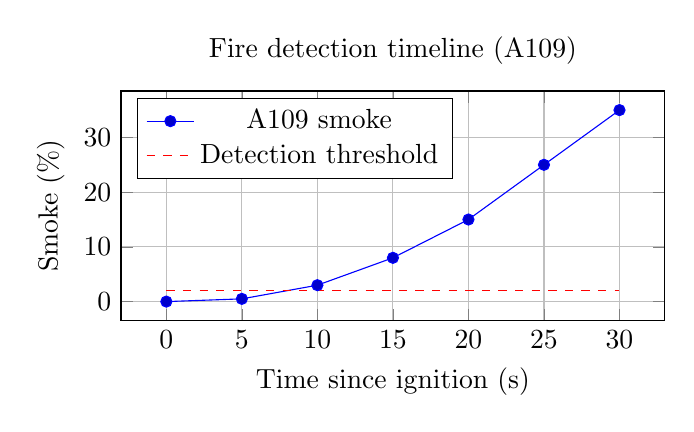
\begin{tikzpicture}
\begin{axis}[width=0.7\linewidth,height=4.5cm,
  xlabel={Time since ignition (s)},ylabel={Smoke (\%)},
  title={Fire detection timeline (A109)},grid=both,
  legend pos=north west]
\addplot coordinates {(0,0) (5,0.5) (10,3) (15,8) (20,15) (25,25) (30,35)};
\addplot[dashed,red] coordinates {(0,2) (30,2)};
\legend{A109 smoke,Detection threshold}
\end{axis}
\end{tikzpicture}
\end{center}

The agent detected fire within 15--20\,s in repeated tests, well within the 60\,s budget.

\textbf{Scale (NFR-01, NFR-03).} The full system runs 950 rooms $\times$ 3 sensors = 2,868 sensors at a 5\,s interval, producing $\approx$570 readings/s sustained. TimescaleDB handled this without backpressure. The Grafana dashboard remains responsive with per-floor filtering.

\textbf{Edge deployment (NFR-04).} The ONNX model (1,695\,KB) runs on the Raspberry Pi 400 (aarch64, 4\,GB RAM):
\begin{itemize}\tightlist
  \item Normal readings → not fire ✓
  \item Fire readings → fire ✓
  \item False alarm → fire (expected---16\% leakage, hence the LLM second pass)
\end{itemize}

\textbf{Graceful degradation (NFR-02).} With the LLM endpoint unreachable, the fallback agent detected fire and activated sprinklers within two detection cycles ($\approx$20\,s), confirmed by 2 unit tests.

\textbf{Honest critique.} The 73\% normal accuracy on real data means the isolation forest triggers too often on baseline readings at scale, which is why the threshold filter (smoke $>$ 2, CO $>$ 5, temp $>$ 25) was added before the LLM call. Without it, the agent would make $\sim$50 LLM calls per tick instead of 1--3. The temperature baseline also drifts higher than expected ($\sim$48°C without fire) due to cumulative occupancy heat; the heat coefficient was reduced from 0.02 to 0.001 but remains an area for improvement. Finally, the actuators are registered in BuildSim but not individually polled at scale (1,100 processes would overwhelm the HTTP client); in a real deployment, actuators would communicate via a local bus, not HTTP.


%% ============================================================================
\section{12. Dashboard}
%% ============================================================================

Two Grafana dashboards are used:

\textbf{Operations dashboard} (for the building manager):
\begin{itemize}\tightlist
  \item \textbf{Row 1:} Active rooms count, max smoke/CO/temperature (color-coded green→yellow→red), active fires table
  \item \textbf{Row 2:} Top rooms by anomaly---only rooms exceeding thresholds are shown (empty when calm, populated during fire)
  \item \textbf{Row 3:} Fire room correlation (all 3 sensors for the most-affected room), sensor statistics table (sortable by max value)
  \item \textbf{Row 4:} Fire events log with response plans, fire spread bar gauge (top 10 rooms by smoke)
  \item \textbf{Row 5:} Anomaly count, agent response time, sprinklers active, rooms per floor
  \item \textbf{Filters:} Floor dropdown (All / level0 / level1 / level2), room multi-select
\end{itemize}

\textbf{Technical dashboard} (for engineers):
\begin{itemize}\tightlist
  \item Pipeline health (readings/min per floor), throughput per sensor type
  \item Database size (row counts), detector accuracy metrics
  \item Links to Phoenix (LLM traces), ClearML (training experiments), BuildSim (3D viewer), Swagger UI (control API)
\end{itemize}

\diagramslot{Dashboard screenshots: operations dashboard during fire, technical dashboard}

The operations dashboard's key design principle: \textbf{empty panels = building is safe}. An operator glances at the dashboard and sees green stat panels + empty anomaly charts = everything normal. When fire starts, panels turn red, anomaly charts populate, and the fire events table shows the agent's response plan.


%% ============================================================================
\section{13. Risks and critical reflection}
%% ============================================================================

\textbf{Sensor degradation model is symmetric.} All rooms get the same noise parameters. A real building would have older sensors in some rooms (more drift), recently-replaced sensors in others, and environmental factors (humidity, dust) that vary. The data-quality handling would benefit from per-sensor calibration profiles.

\textbf{The LLM is a single point of intelligence.} The fallback works, but it is less capable: it cannot reason about ``smoke without CO means false alarm.'' A production system would want a lightweight local model (e.g., a small classifier trained on labelled fire events) as a middle tier between the isolation forest and the LLM.

\textbf{Actuators are modelled, not individually polled.} At 950 rooms, running 1,100 individual actuator processes (each polling BuildSim via HTTP every second) overwhelmed the connection pool. The solution was to register actuators in BuildSim but model their behaviour in the physics engine. A real building uses a local fieldbus (BACnet, Modbus), not HTTP, so this limitation is simulation-specific.

\textbf{Temperature baseline drifts.} Occupancy heat accumulates faster than envelope loss dissipates, causing baseline temperatures to rise above realistic levels ($\sim$48°C) without fire. The coefficient was reduced but not eliminated. A production physics model would include HVAC cooling as a negative feedback term.

\textbf{Cross-floor fire response is demonstrated but coarse.} The system unlocks doors on all floors when fire is detected on any floor. A more sophisticated approach would identify which stairwells are affected and only modify routes through those stairwells, leaving unaffected paths open. The evacuation planner supports this (it blocks specific rooms), but the LLM's plan generation does not yet exploit it fully.

\textbf{What would be done with more time:}
\begin{itemize}\tightlist
  \item Per-sensor calibration profiles for more realistic degradation
  \item A lightweight local classifier as a middle tier between isolation forest and LLM
  \item HVAC integration: the physics model already has the sprinkler feedback loop; adding HVAC would enable smoke extraction and pressure management
  \item Stairwell-specific evacuation: block only affected stairwells, not all doors
  \item Live Grafana-to-LLM integration: operator asks ``why did you activate sprinklers in A108?'' and gets a natural-language explanation from the agent's decision log
\end{itemize}

\begin{longtable}[]{@{}
  >{\raggedright\arraybackslash}p{0.30\linewidth}
  >{\raggedright\arraybackslash}p{0.20\linewidth}
  >{\raggedright\arraybackslash}p{0.44\linewidth}@{}}
\toprule
\textbf{Risk / assumption} & \textbf{Impact} & \textbf{Mitigation / decision} \\
\midrule
\endhead
LLM unavailable & No contextual reasoning & Rule-based fallback (tested, NFR-02) \\
Sensor drift undetected & Slow false alarm rise & Stuck-sensor detection via gateway; drift detection planned \\
MQTT broker is SPOF & Sensor data stops flowing & Persistent sessions; restart policy; sensors buffer briefly \\
Simulated physics is optimistic & Detection times may differ in real buildings & Reported relative to requirements, not absolute \\
Single-threaded agent & Caps rooms per tick & Batch polling via equipment list; shard by floor if scaled \\
\bottomrule
\end{longtable}


\end{document}